\documentclass[12pt, a4paper, oneside]{article}\usepackage[]{graphicx}\usepackage[]{color}
%% maxwidth is the original width if it is less than linewidth
%% otherwise use linewidth (to make sure the graphics do not exceed the margin)
\makeatletter
\def\maxwidth{ %
  \ifdim\Gin@nat@width>\linewidth
    \linewidth
  \else
    \Gin@nat@width
  \fi
}
\makeatother

\definecolor{fgcolor}{rgb}{0.345, 0.345, 0.345}
\newcommand{\hlnum}[1]{\textcolor[rgb]{0.686,0.059,0.569}{#1}}%
\newcommand{\hlstr}[1]{\textcolor[rgb]{0.192,0.494,0.8}{#1}}%
\newcommand{\hlcom}[1]{\textcolor[rgb]{0.678,0.584,0.686}{\textit{#1}}}%
\newcommand{\hlopt}[1]{\textcolor[rgb]{0,0,0}{#1}}%
\newcommand{\hlstd}[1]{\textcolor[rgb]{0.345,0.345,0.345}{#1}}%
\newcommand{\hlkwa}[1]{\textcolor[rgb]{0.161,0.373,0.58}{\textbf{#1}}}%
\newcommand{\hlkwb}[1]{\textcolor[rgb]{0.69,0.353,0.396}{#1}}%
\newcommand{\hlkwc}[1]{\textcolor[rgb]{0.333,0.667,0.333}{#1}}%
\newcommand{\hlkwd}[1]{\textcolor[rgb]{0.737,0.353,0.396}{\textbf{#1}}}%
\let\hlipl\hlkwb

\usepackage{framed}
\makeatletter
\newenvironment{kframe}{%
 \def\at@end@of@kframe{}%
 \ifinner\ifhmode%
  \def\at@end@of@kframe{\end{minipage}}%
  \begin{minipage}{\columnwidth}%
 \fi\fi%
 \def\FrameCommand##1{\hskip\@totalleftmargin \hskip-\fboxsep
 \colorbox{shadecolor}{##1}\hskip-\fboxsep
     % There is no \\@totalrightmargin, so:
     \hskip-\linewidth \hskip-\@totalleftmargin \hskip\columnwidth}%
 \MakeFramed {\advance\hsize-\width
   \@totalleftmargin\z@ \linewidth\hsize
   \@setminipage}}%
 {\par\unskip\endMakeFramed%
 \at@end@of@kframe}
\makeatother

\definecolor{shadecolor}{rgb}{.97, .97, .97}
\definecolor{messagecolor}{rgb}{0, 0, 0}
\definecolor{warningcolor}{rgb}{1, 0, 1}
\definecolor{errorcolor}{rgb}{1, 0, 0}
\newenvironment{knitrout}{}{} % an empty environment to be redefined in TeX

\usepackage{alltt} % Paper size, default font size and one-sided paper
%\usepackage[dcucite]{harvard}
\usepackage{tikz}
%\usetikzlibrary{shapes, shadows, arrows}
\usepackage{rotating}
\usepackage{amsmath}
%\usepackage{setspace}
\usepackage{pdflscape}
\usepackage[flushleft]{threeparttable}
\usepackage{multirow}
\usepackage[comma, sort&compress]{natbib}% Use the natbib reference package - read up on this to edit the reference style; if you want text (e.g. Smith et al., 2012) for the in-text references (instead of numbers), remove 'numbers' 
\usepackage{graphicx}
\graphicspath{{./Figures/}} % Specifies the directory where pictures are stored
%\bibliographystyle{plainnat}
%\usepackage{listings}
\bibliographystyle{agsm}
\usepackage[colorlinks = true, citecolor = blue, linkcolor = blue]{hyperref}
%\hypersetup{urlcolor=blue, colorlinks=true} % Colors hyperlinks in blue - change to black if annoying
\IfFileExists{upquote.sty}{\usepackage{upquote}}{}
\begin{document}
%\renewcommand[\harvardurl]{URL: \url}
\title{Carry trade, sudden stops and instability in emerging markets}
\author{Rob Hayward\footnote{University of Brighton Business School, Lewes Road, Brighton, BN2 4AT; Telephone 01273 642586.  rh49@brighton.ac.uk.} and Jens H\"{o}lscher\footnote{Bournemouth University, Executive Business Centre, 89 Holdenhurst Road, Bournemouth, BH8 8EB; Telephone 01}}  
\date{\today}
\maketitle
\begin{abstract}
International financial crises disproportionately affect emerging economies.  These crises are frequently the result of the unwinding of carry-trade positions.  The carry-trade is the attempt to take advantage of the breakdown of uncovered interest parity by borrowing low interest rate currencies, exchanging for higher rate currencies and taking the interest rate differential less the depreciation of the investment currency against the funding unit.  If there is fear that the investment currency will depreciation, this can trigger a sudden-stop or reversal of inbound capital flows as funds seek to exit the carry position before the collapse.  A Hidden Markov Model uses the observed returns from the carry-trade to estimate the unknown probability of a shift from a state of financial stability to one of instability. This model is then used to assess the way that rising risk aversion affects the probability of a financial crisis. While the Czech Republic,  Hungary and Bulgaria are very sensitive to international financial conditions, Poland and Romania are relatively immune.  
\end{abstract}

\section{Introduction}
As the size of international capital flow has increased in absolute terms and relative to the expansion of the trade in goods and services, it has also become subject to less regulatory constraint. Economic authorities in emerging economies have struggled with financial instability that has an international source.  An inflow of capital from abroad may appear attractive but its arrival can inflate the price of goods and assets; it can shape institutions, economic development and political opinion; and the inflows can disappear even more swiftly than they arrive.  %Transition and emerging economies have been particularly affected by international financial crises.  %The financial systems of transition and emerging economies are less developed than those of the the international finance centres and therefore there is scope in these countries for the financial sector to increase in size and relative to overall level of economic activity.  This process can attract financial entities from more developed economies. \citet{ONBcarry} and \citet{EBRD} survey the expansion of Euro area banks into the Central and Eastern European trasition economies; \citet{Gabor} discusses the political economy of this \emph{financialization} where the financial system expands to new sections of the economy.  

%Bernanke speaking to Joint Economic Committee on 22-May-13.  Speaking about moderating asset purchase, but not yet. 
%http://www.federalreserve.gov/newsevents/testimony/bernanke20130522a.htm

International financial conditions in the immediate adtermath of the 2007-08 Global Financial Crisis (GFC) have fuelled the growth of investments in transition and emerging economies by providing large amount of funding-currency liquidity in the financial systems of developed economies.  However, any steps towards \emph{normalisation} of monetary policy in developed nations have flows reversal and have raised concern about the financial stabilitu of merging economies.  There are three  potential triggers for such a reversal:  US monetary policy, international risk aversion and international liquidity. 

We used a Hidden Markov Model (HMM) to determine financial conditions from the returns achieved by the carry-trade invested in emerging European countries. In most cases, a model with two regimes explains the data better than those with one or three.  We estimated a transition matrix that identifies the probability of switching from a position of calm to one of financial crisis. We also estimated the transitional matrix probabilities conditional on the level of international risk, US interest rates and banking liquidity.  This is used to identify the way that these factors affect the vulnerability of countries to international shocks.    % Need to link this to the use of risk factors (portfolio country risk).    
  
\section{Financial crisis and sudden stops}
International financial crises have been a prominent impediment to emerging economy development in the last thirty years.  Globalisation of financial markets encourages capital to move from one opportunity to another. The term \emph{sudden stop} has been used to express the shock that is suffered once these capital flows are curtailed out cut back, see \citet{DornbuschSS}, \citet{CalvoSS} and \citet{KrugmanSS}.    %The gradual increase in risk followed by a sharp reversal lends itself to a model that takes more than one regime. %There is a focus on the factors that may make a country more or less vulnerable to sudden-stops with debate over the role that openness to trade \citet{Cavallo20081430} and overseas banking liabilities pose from \citet{calvo2004empiric}.   
 
  Following the Global Financial Crisis (GFC) the flow of finance to emerging economies has accelerated as a consequence of liquidity stoked by quantitative easing in key financial centres and by emerging market investment opportunities.  However, since the intial move towards cutting back expansionary monetary policy that was indicated by Fed Chairman Bernanke in May 2013, this has evolved into an ebb and flow that is influenced by international events.  Three major internatioanl factors have been identified as increased US interest rates, elevated internatioanl risk aversion and funding conditions in international banks. These factros seem to have as much effect on emerging economy vlunerability as the individual circumstances of the emerging states.  As a consequence,  rising international risk aversion, higher interest rates and cutbacks in liquidity have been added to the role that openness to trade (\citet{Cavallo20081430}) and overseas banking liabilities (\citet{calvo2004empiric}) pose to emerging economy stability.   

The relative importance of each of these three internatonal factros has come under recent investigation.  \citet{Cerutti2014} ask three questions:  what drives global liquidity; where does the global liquidity cycle originate; how can the recipient countries manage exposure to global liquidity?  They conclude that while the US drives the global liquidity cycle through its monetary policy, other financial centres (particularly in European) affect the financial cycle through the conditions of their banks. Their work suggests that global liquidity is affected by global financial conditions rather than monetary policy.

%\href{http://www.federalreserve.gov/pubs/feds/2014/201446/201446abs.html}{Fed Paper} 
Flight-to-Safety (FTS) is the term used to describe capital flows towards international financial centres and relatively safe assets, \citet{FTS} discover that FTS are relatively rare events. Their study of of 23 countries identifies FTS in less than 3\% of the sample of daily data that runs from January 1980 to January 2012.  In a contrast to other work, they find that most of the events are country specific (they characterise only 25\% of the events as "global") and are associated with an increase in the VIX index and the TED spread.\footnote{The VIX is an index of implied volatility on options from the S\&P 500 index.  It is commonly used as a measure of international risk aversion as it signals increased demand by fund managers for option protection of their equity portfolio.  See \citet{VIX}, \citet{GoldmanVol} and \citet{Diamond} for fuller details.The TED spread is the spread between the treasury bill and the Euro-dollar rate.  It is used as a market measure of perceived credit risk of financial institutions as it records the risk premium that investors require to lend to banks relative to the risk-free rate.}   %These FTS eposodes are also associated with lower levels of consumer sentiment, appreciation of the  Yen, Swiss franc and US dollar funding currencies. %Financial, basic materials and industrial industries under-perform in FTS periods while telecoms outperform; money market instruments, corproate bonds and commodity prices (other than precious metals) face abnormal negative returns, hedge funds (particularly "event-driven" display negative FTS beta.  Liquidity deteriorates on FTS days in bond and equity markets. Economic growth and inflation decline in the year after a FTS event. 

%\href{http://www.imf.org/external/pubs/cat/longres.aspx?sk=41655.0}{IMF:  Impact of Fed tapering annoncement on emerging markets}.  

Consistent with the evidence of an interplay between monetary policy and international risk, and between domestic and international factors, \citet{Ahmed2014} run a multivariate panel of gross and net capital flows before and after the financial crisis, showing that economic growth, interest rate differentials and the level of global risk appetite are all important determinants of private capital flows to emerging markets.  They also suggest that capital flows have been more sensitive to interest rate differentials since the financial crisis of 2007-08. There is also some evidence that quantitative easing has had some effect on capital flows. 

\citet{IMFLatam} use a panel vector autoregression (VAR) method to identify the influence of US monetary policy since 1990 on capital flows to 38 emerging economies, finding evidence that the end to Federal Reserve purchase of government bonds under the quantitative easing programme, while not necessarily leading to capital outflow, could generate \emph{new risk premium shocks} with investors requiring a higher rate of return and therefore lower asset prices.

While the origin of international financial crisis may be international the effects may vary by asset class and country in a variety of ways.  Using daily data on exchange rates, stock prices and emerging market bonds, \citet{Tapering} find that exchange rates and bonds are less affected by international liquidity shocks than stock markets.  They also find that stronger domestic macroeconomic fundamentals, more prudent financial policy and deeper financial markets provide some insulation against US monetary policy shocks.

The flow of international bank lending is more difficult to measure but seems to host most of the speculative activity.  One specific part of the range of international capital flows that has attracted particular attention because it is associated with speculation is the \emph{carry-trade}.  This is the attempt to take advantage of the break down in \emph{uncovered interest parity} (UIP).\footnote{See \citet{fama1993common}, \citet{FrootFrankelFDB} and \citet{Hayward2013} for an overview of the failure of UIP.  This provides a rationale for borrowing low interest rate currencies and investing in units with a higher return.} Most of the explanation of UIP revolve around the idea that what is supposed to be an excess return is actually a return for taking \emph{crash-risk}.  This is the small probability of a large, probably fatal, loss. This is the equivalent of the sudden-stop for the investor. The attempt to exit the investment in the emerging market causes the fall in the value of the investment currency that is to be avoided. 

\citet{BrunnermeierCarry} analyse a sample of carry trades and find that the returns are characterised by negative skew and a larger than normal risk of extreme loss; \citet{JurekCrash} assesses the cost of purchasing option protection against crash-risk and shows that the price of out-of-the-money puts covers a proportion of the excess returns that seem to be generated by the carry-trade; \citet{Hayward2013} compares carry returns in period of stable and periods of crisis (as measured by elevated levels of the VIX index).  Carry-returns are negative, skewed and fat-tailed when international risk aversion is heightened, but a more normal, positive return when conditions are stable. 

\citet{NYFedtaper} consider the effect of changes in global risk aversion on the carry-trade.  They find that the initial signal from the US central bank in Fed Chairman Bernanke's May 22 2013 testimony to Congress coincide with an increase in global risk aversion which affected global asset prices. %They use the approach presented by \citet{MertensSVAR} to estimate the effect of policy changes by using a two-stage least squares appraoch to identify the SVAR model of asset price changes.  
By identifying the performance of exchange rates without a change in risk aversion, they suggest that nearly half of the depreciation of a basket of 45 carry-trade currencies with the largest one-month interest rate relative to a basket of the US dollar and other equally low rate currencies is explained by this increased risk aversion. Nearly all the decline in Emerging market equities is attributable to the increase in risk aversion.

There is evidence that the international financial cycle is increasingly global.  See \citet{Rey2013}, \citet{Obstfeld2014} and \citet{Bruno2014} for example.  %\href{http://www.voxeu.org/article/primer-global-liquidity}{VOX: GLobal Financial Liquidity}. 
There is evidence the correlation of cross-border credit growth has risen since the 1990s and that funds increasingly flow from the financial centres to the rest of the world. For \citet{Cerutti2014}, credit and liquidity contractions in  the US, Euro zone, UK and Japan affect the rest of the world.   This is what they call \emph{global funding liquidity}, a feature that affects financial conditions globally by transferring credit supply in financial centre economies through the provision of cross-border credit.

The aim here is to assess how vulnerable contries are to a financial crisis, to model this as a regime-switch and to quantfy how far changes in international risk factors can alter the probability of a financial crisis in indevidual countries.  This can then be used to help understand some of the factors that may increase risk of financial crisis.  The rest of this paper proceeds as follows: the Section \ref{secref:HMM} presents the model; Section \ref{secref:res} presents the results; Section \ref{secred:con}


%Do the next two paragraphs set up the dicotomy between the domestic factors and the international (flight-to-quality) factors?  THere are a range of facts:  EM debt rose from 650bn in 2001 to 6.9tn in 2013 according to BIS data.  

%\subsection{The instability cycle}
%The aim of this study is to understand more about the evolution of internatonal financial instability by studying the carry trade in a number of European transition and emerging economies. There are two related areas of interest:  the factors that trigger a crash, reversal or sudden-stop; the way that the financial system evolves to the point where the crash is likely to take place.  There have been a number of attempts to identify levels of finacial risk.  This has clearly become even more of an issue since the financial crisis.  For example, \citet{IFCMeasure}.  The IMF have developed a range of \emph{Financial Soundness Indications} (IMF 2006).     Also - Hawkins and Klau (2000), Nelson and Perli (2005) and Gray et al (2007).  There are six main strands:  the real sector, including fiscal position and inflation; the corporate sector, specifically the level of debt and overseas exposure; the ability of the household sector to weather downturns; the external sector, including the foreign exchange position and the capital account; the financial sector; finacial markets. 

%A number of studies applied the early warning indicator methods initially developed in the literature for currency and balance of payments crises to banking crises. Earlier work includes, among others, Calvo et al (1993), Eichengreen et al (1996), Turner and Goldstein (1996) Frankel and Rose (1996). Demirgüç-Kunt and Detragiache (1997) use a multivariate Logit approach to identify determinants of banking crises in a large panel of developing and industrialised countries: slow GDP growth and high inflation, vulnerability to sudden capital outflows, low liquidity in the banking sector, a high share of credit to the private sector, past credit growth, explicit deposit insurance and weak institutions. Kaminsky and Reinhardt (1999) identify early warning indicators of twin (banking and balance of payments) crises, such as credit and equity prices, by looking at the ability of such variables to predict crises 12 or 24 months a, while minimising the noise3  to signal ratio. Borio and Lowe (2002) and Borio and Drehmann (2009) build on the techniques developed by Kaminsky and Reinhardt (1999). Like the latter, they define threshold values for the indicators, but unlike them, they look at cumulative processes rather than just growth rates over one year, they use ex ante information (ie information which was available to the policymaker prior to the crisis) and, for the first time, they consider combinations of indicators and look at multiple time horizons. BIS Goodhart 2006%

%However, While measuring debt-to-equity ratios and the scale of bank lending may provide some indication about the regime that is in place, this is imprecise and it is clear that financial services business evolve in ways that make loan counting  inadequate.The recent financial crisis showed that innovations like \emph{Collateralised Debt Obligations (CDO)} can allow an increase in debt that does not directly in bank lending. 

\section{The Hidden Markov Model}\label{secref:HMM}
\subsection{The evolution of financial instability}
International financial risk and the carry-trade are beset by \emph{peso problems}. Peso problems are cases where there is  potential for discrete shifts in the distribution of variables.  This can affect expectations, risk-premia and asset pricing models. In \citet{evans199621}, for example, if $s_t$ is the log of US dollars in terms of Mexican peso and the peso is fixed at 0.08 dollars with information set $\Omega_t$, this is state $s^0$ with a expected probability $\pi$ at time $t$, which is a fixed period ahead, that there will be a discrete exchange rate adjustment to $s^1$, the expected depreciation is 
\begin{equation}
E[s_{t+1}|\Omega_t] = \pi_ts^1 + (1 - \pi_t)s^0
\end{equation}
Therefore, the difference between the realised and expected rate is 
\begin{equation}
s^0 - E[s_{t+1}|\Omega_t] = \pi_t(s^0 - s^1)
\end{equation}

%A common problem in estimating economic models is that the parameters do not tend to be stable over time.  A HMM can be used to model a range of cases that can span a simple transition from one state to another, switching between multiple regimes with varying parameters towards the extreme where the number of regimes mean that system is close to having time-varying parameters (TVP).  

Expectations are continually confounded though they are not formed in an irrational way. In these cases, modelling that identifies the two regimes and the probability of switching between them will help to capture the non-linear nature of the relationship and will allow a range of cases that can span a simple transition from one state to another to an extreme of multiple states where parameters are close to time-varying.  

%This may be addressed through a \emph{theshold model}. 

\citet{hamilton1988rational} used a Hidden Markov Model (HMM) to incorporate discrete changes in expectations about Fed policy to make a closer match between the expectations theory and the term structure of interest rates.  This technique assumes that there are hidden or unobserved regimes and that the adjustment from one state to another is governed by a set of probabilities.  \citet{Hamilton1989} also analysed the performance of postwar US GNP with adjustments from periods of positive to negative growth. The regime shift is modelled as a first-order Markov process.  In other words, state $S_t$ depends only on the previous state $S_{t-1}$, with given probabilities that the state will switch or remain unchanged.  The parameters of an ARIMA representation of US GNP shift between the two regimes so that in periods of recession the underlying growth rate is three percentage points lower than it is during the expansionary period.   
%\emph{The peso problem} describes a range of cases where there is a large, descrete shift or \emph{jump} in the system.  This is particularly relevant to the carry-trade as one explanation for the evidence of a breakdown in UIP is that exchange rate expectations cannot be modeled by taking the average of past realisations. 


%The raw model just assume that there are three states with random allocation of the starting values.  However, the initial estimates of the regime parameters can come from the estimates made in the doctorate using the crash and caution identification from the VIX; the initial estimates of the priobabilities of each state can come from the percentage of each state in the final version of the model that is run without initial estimates.  

%I think that $\theta_1$ on page 4 of the depmixS4 vignette is the parameter that nees to be set. 

%At the top of page 10 of the vignette, there is an example of how the transition matrix may be augmented by a model.  I do not understand this fuilly, but it may be possible to link the transition to the VIX index.  Obviously, there is some risk of circularity here. Anyway, it may be useful to compare the difference. 


\citet{schaller1997regime} extend the Hamilton model to assess stock returns in two regimes, uncovering strong evidence of regime-switching between bull and bear markets in the mean and variance of US stock returns.  They also find that that the response of stock returns to the price-dividend ratio is asymmetric as adjustment is much swifter during the bull market phase; \citet{dueker1997markov} use a model that switches from periods of low to high volatility. Markov models switching models are also typically used to understand the evolution of credit risk.  A transition matrix with probabilities derived empirically provides the expectation that a rating will change from one level to another.  This can be rolled forward to assess the likelihood of a default and used to incorporate credit risk in the valuation of bonds.  As an extension of this,  \citet{frydman2008credit} use a \emph{mixture model}, where the underlying probabilities of adjustment come from two underlying sub-models of company type, against the alternative of a pure Markov chain. The observed rating changes relate to two different underlying Markov chains representing the evolution of credit ratings.  There is a heterogeneity that seems to depend upon the industry.  For example, ratings of firms in the retail and wholesale trade sectors tend to be more dynamic than the others. 


%Agn Timmerman (2011)
%Looking at how abrupt changes in regime can lead to changes in the way that the system works.  The different regimes can be associated with different underlying distribution of returns.  This can allow the understanding of the non-liner and non--normal distribution within  normal or linear framework.  At the extreme, the regime switch model can incorporate a \emph{jump model} with one change, and can also be associated with time-varying parameter models that have a large number of regimes.

%The broad framework for the method is to model a discrete state $s_t \in %\{0,1,\dots k \}$
%\begin{equation}
%y_t = \mu_{s_t} + \phi_{s_t} y_{t-1} + \sigma_{s_t} \varepsilon_t, \quad %\varepsilon_t \sim iid(0,1) 
%\end{equation}

%The process governing the underlying regime must also be defined. 

%\begin{equation}
%Pr(s_t = 0| s_{t-1} = 0) = p_{00} \quad \text{and} \quad Pr(s_t = 1| s_{t%-1} = 1) = p_{11}
%\end{equation}

%More generally, the transition could be time-varying and could be dependent on the time spent in the regime.  See Durland and McCurdy (1994) for example of the probbilities  in the transition matrix being related to time. The longer the systemm has remained in the build phase, the greater the risk of crash.  Remember that the crash phase is a period when there is risk of a sharp reversal.  

%See Diebold, Lee and Iinbch (1994) for examples where the transition probabilities depend on some other state variables.  For example, the interest rate spread.   Could the VIX index or other factors be used?  Vix index would indicate heightened international tension as one element that affects the probability of transforming from one state to the next.  An elevated VIX is an indication of the heightened international risk premium.  This may increase the probability that the regime switches from carry build to crash.  This is a theme that could be related to the bubble bursting so any information that improves the ability to identify bubbles bursting would be beneficial.  


%There are two states of the world:  crisis and moderation.  If the system is in a crisis, it stays there with probability p; it switches to moderation with probability $1-p$.  If in moderation, the system stays there with a probability q and switches to crisis with probability $1-q$.  If the probabilities change over time, there is no longer a \emph{homogenous Markov Chain}. Ghysels has a seasonal dummy for the probabilities that represent the months or quarters.  

%Can the probabilities change over time?  This may be the result of changes in the resilience of the financial system. 
%\href{http://members.home.nl/jeroenvermunt/dias2010.pdf}{Mixture Hidden Markov Models} Hidden models help to calafify the regime under which securities trade. Model takes into account the unobserved hetrogeneity across time. This could could be extended to space (for different countries).  Is it possible to estimate a panel? 

%Can the systemm be used to compare to fixed and floating exchange rates. 

%The use of the regime-switch allows the transition from one regime to another to be the result of something that is more than just a deterministic process. There are a number of ways that this model could be expanded.  Dueker has a model where the degrees of freedom from a Student-t distribution change with the regime.  

%An alternative way to look at this would be to use a TAR mode.  

%There are three main ways that the evolution of international financial risk can be modelled.  The first is through a one-off transition from calm to crisis. This represents a world there has been some major event that has transformed the system and where there has been a permanent adjustment from one regime to another.  This is a one-off switch that may be a function of political or policy changes that are permanent. For example, this could be caused by a move from a fixed exchange rate to something more variable or another type of shift in monetary policy regime.   

%The second and moris a two-regime model where there is a switch between periods of calm and crisis.  This is  a relatively simple system where the interest is in the factors that can trigger an adjustment from one regime to another.  A more sophisticated version of this is the third model were there is an evolution of the system from a position of calm, through a time when speculative positions are build and then into a crash. 

%The third is a more sophistocated model that would add further dynamics. 

%The relatively simple model that switches between periods of calm and crisis has been discussed by \citet{DornbuschSS}, \citet{CalvoSS} and \citet{KrugmanSS}.  The term \emph{sudden stop} emphasises the importance of the inflow of international capital that takes place before the disruptive effects of reversal.  

%other references 
 %Abiad, A., 2003. Early-Warning Systems: A Survey and and a Regime-Switching Approach. IMF Working Paper No.03/32. International Monetary Fund.
 %Aziz, J., Caramazza, F., Salgado, R., 2000. Currency Crises: In Search of Common Elements. IMF Working Paper No.00/67. International Monetary Fund
 %Calvo, G., 2000. Balance-of-Payments Crises in Emerging Markets: Large Capital Inflows and Sovereign Governments, in: Krugman, P. (Ed.), Currency Crises, University of Chicago Press, Chicago, Illinois,
% \href{http://mpra.ub.uni-muenchen.de/383/}{http://mpra.ub.uni-muenchen.de/383/}

%Minsky's \emph{Financial Instability Hypothesis} (FIH) presents a model of endogenous financial crisis where a period of economic calm creates the conditions for more adventurous and risky financial behaviour that increases the fragility of the system \citet{MinskyStabilising, MinskyKeynes, MinskyFIH, MinskyLongerWaves}.  Minsky identified three phases of financing:  hedge, speculative and Ponzie.  

%In the first of these the system is stable as lending is not excessive, borrowers are cautious and revenues are generally sufficient to ensure that repayments of principal and interest can be made from current income.  This period may be framed by memories of past financial crisis and the economic hardships that are associated with it.  Violent economic shocks are among the range of possible outcomes that can readily be envisaged by creditors and debtors, encouraging them to be cautious and risk-averse. 

%However, in the absence of economic shocks these memories of hardship fade further into the background and all parts of the economic and financial system become more prepared to take risks.  Lending becomes more speculative; decision-making gives less weight to the possibility of extreme outcomes and put more emphasis on the immediate experience of economic calm.  The increase in lending tends to improve immediate economic conditions:  business investment and consumer spending rise if lending is broad-based; asset prices will appreciate where lending is directed towards financial investment.  The increase in economic activity that comes from this expansion in credit will feedback to improve immediate economic conditions, exacerbating the sense of well-being and undermining the arguments of those preaching more cautious behaviour.  Positive feedback effects cause a non-linear relationship between credit growth and economic activity and between credit and asset prices. 

%\citet{BernankeGertler}, \citet{Bernanke1999chapter} and \citet{Azaraidis} present models where there is a non-linear relationship between  the provision of credit and the level of economic activity. \citet{BernankeGertlerAgency} show how balance sheet dynamics can affect the business cycle through a reduction in the agency cost of business investments and \citet{Balke} has a non-linear model of credit shocks.  \citet{Avdjiev2014} use a three regime Threshold-Vector-Auto regression (TVAR) to identify the non-linearities in credit market shocks.  They find that credit shocks have the greatest impact when output growth is above its long-term trend. 

%While credit becomes more plentiful, household and business managers become more optimistic.  There is evidence that decision-making tends to favour outcomes that are more recent, apparent or those that that can be more easily envisaged (see for example, \citet{KTAvailability} and \citet{Schwartzavailability} for some evidence on the \emph{availability heuristic} and related literature).   % more required or footnote? 

%In this way, the repayment of loans becomes increasingly dependent on the continuation of above-normal economic conditions or the appreciation of asset prices.  If this process is allowed to continue, a speculative frenzy can take hold.  Economic agents are dragged into the euphoria as households compete with the conspicuous consumption of their neighbours, businesses investment expands to increase capacity and market share in the face of booming demand, while property and financial market speculators redouble their bets.  \citet{BrunnermeierLiquidity} show how the link between the availability of credit for investors and the level of liquidity in financial markets can create \emph{liquidity spirals}.   They note that the capital of speculators can drive market liquidity, risk premia and asset prices.  The ability to be able to borrow against collateral is particularly important here.  As asset prices increase, the ability to borrow against their value raises the amount of trading credit that is available.  

%The conditions are now in place for the bubble to burst in a violent reversal.  \citet{FisherBD, FisherDD} explained the way that \emph{debt-deflation} could create a ricochet between the financial and real sectors of the economy with a decline in the availability of credit exacerbating the financial strain on households and business, helping to reduce household and business spending thereby raising the quantity of bad loans and the sense of caution at financial institutions. In financial markets, credit and liquidity disappear and the decline in asset value affects the ability of institutions to raise funds.  Fire sales in illiquid markets exaggerate the fall in prices. \citet{ReinhartRogoff} reveal how credit booms help to explain the breadth and depth of post-boom recessions.  The catalyst for the collapse is difficult to pin down as the build up to the excess is fragile.  See \citet{Gorton2013} and \citet{BrunnermeierLiquidity} again for financial market effects. The economic consequences are profound.  


\subsection{The HMM model}
Though {\citet{CalvoSS} defines the sudden stop as a one movement of net capital flows to two standard deviations from the mean and a return to one standard deviation from the mean, a financial crisis is hard to define.  In situations like this where the underlying financial regimes are not observable, the Markov model is not sufficient to fully describe the process. It may nonetheless be possible to identify a probabilistic relationship between something that is observable and that which is to be defined.  In this case, the carry-trade returns are observable and are used to identify the underlying financial regime.  This is described as a \emph{Hidden Markov Model (HMM)}. 

Figure \ref{figref:HMM2} gives an overview of the system.  The HMM has three components: $\pi, A, B$ where,

\begin{itemize}
\item The prior model: $P(S_1 = n| \theta_{prior})$ $(\pi)$
\item The transition model: $P(S_t| S_{t-1}, \theta_{trans})$ $(A)$
\item The response model: $P(Y_t| S_t, \theta_{resp})$ $(B)$
\end{itemize}

Where there are $n$ states or regimes; $y_t$ are the observed carry-trade returns; and $\theta_{prior}$, $\theta_{trans}$ and  $\theta_{resp}$ are the parameters of the prior, transition and response models respectively. The unobserved financial regimes are modelled as a Markov chain that switches from a period of stability to instability.  The returns to the carry-trade are more likely to take particular characteristics according to the underlying regime.   


\begin{figure}
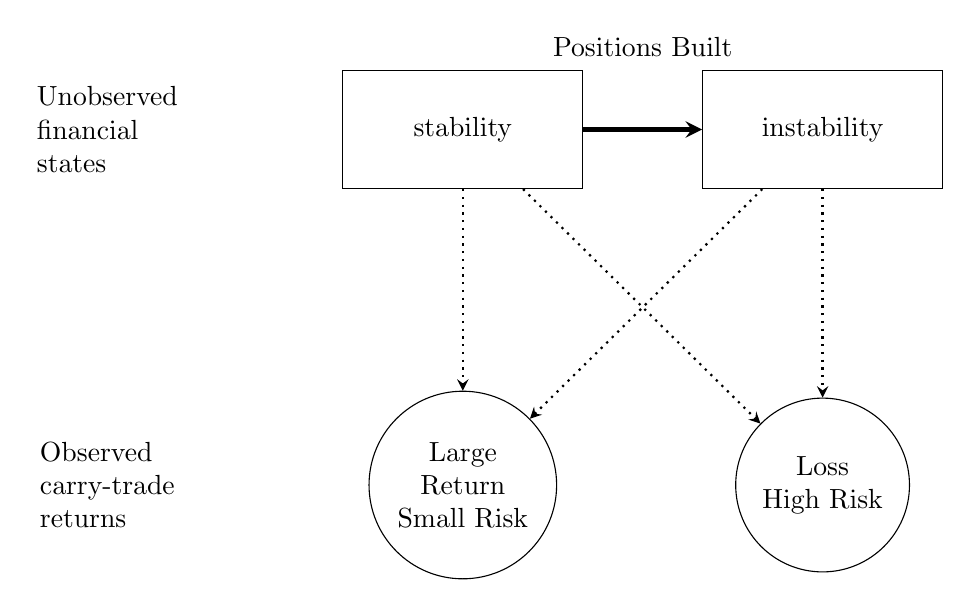
\begin{tikzpicture}
\tikzstyle{decision} = [circle, draw, minimum height = 8mm, 
  text width = 5em, text centered];
\tikzstyle{line} = [draw, -stealth, thick]
\tikzstyle{line2} = [draw, -stealth, ultra thick]
\tikzstyle{line3} = [draw, -stealth, dashed, thick]
\tikzstyle{line4} = [draw, -stealth, dotted, thick]
%\tikzstyle{elli} = [draw, ellipse, fill = red!50, minimum height = 8mm, 
 % text width = 5em, text centered]
\tikzstyle{block} = [draw, rectangle, text width = 8em, 
  text centered, minimum height = 15mm, node distance = 8em]
\node [block](Calm){stability};
%\node [block, left of  = Build, xshift = -5em] (Calm){Calm}; 
\node [block, right  of = Calm, xshift =5em] (Crisis){instability};
\node [decision, below of = Calm, yshift = -10em, align = center]
(Calm2){Large Return \\ Small Risk}; 
\node [decision, below of = Crisis, yshift = -10em](Crisis2) {Loss \\ High Risk};
%\node [decision, below of = Caution, yshift = -10em, align = center](Caution2) 
%{Small \\ Return \\ Average \\ Risk};
%arrows 
%\path [line3] (Calm) -- (Calm);
%\path [line3] (Crisis) -- (Crisis);
%\path [line3] (Crash) -- (Crash2);
\path [line2] (Calm) -- node [yshift = 3em] {Positions Built} (Crisis);
%\path [line2] (Caution) -- node [yshift = 3em]  {Speculative Lending} (Build);
\path [line4] (Calm) -- (Crisis2);
\path [line4] (Crisis) -- (Calm2);
\path [line4] (Calm) -- (Calm2);
\path [line4] (Crisis) -- (Crisis2);
%\path [line4] (Crash) -- (Caution2);
%\path [line4] (Crash) -- (Build2);
\node [align = left, left of = Calm, xshift = -10em] {Unobserved \\ 
financial \\ states};
\node [align = left, left of = Calm2, xshift = -10em] {Observed \\ 
carry-trade\\returns};
%\path [line] (decision1) -| node [yshift = 0.5em, 
%   xshift = 8em] {YES} (process 1);
%\path [line3] (Crash) -- (Caution); 
% 	xshift = -8em] {NO} (process 2);
\end{tikzpicture}
\caption{Two-Regime Hidden Markov Model (HMM)}
\label{figref:HMM2}
\end{figure}




%\begin{landscape}
%\begin{figure}
%\begin{tikzpicture}
%\tikzstyle{decision} = [circle, draw, fill = yellow!30, minimum height = 8mm, 
%  text width = 5em, text centered];
%\tikzstyle{line} = [draw, -stealth, thick]
%\tikzstyle{line2} = [draw, -stealth, ultra thick]
%\tikzstyle{line3} = [draw, -stealth, dashed, thick]
%\tikzstyle{line4} = [draw, -stealth, dotted, thick]
%\tikzstyle{elli} = [draw, ellipse, fill = red!50, minimum height = 8mm, 
%  text width = 5em, text centered]
%\tikzstyle{block} = [draw, rectangle, fill = blue!30, text width = 8em, 
%  text centered, minimum height = 15mm, node distance = 8em]
%\node [block](Build){Build};
%\node [block, left of  = Build, xshift = -5em] (Caution){Caution}; 
%\node [block, right  of = Build, xshift =5em] (Crash){Crash};
%\node [decision, below of = Build, yshift = -10em, align = center]
%(Build2) {High Return \\ Small Risk}; 
%\node [decision, below of = Crash, yshift = -10em](Crash2) {Loss \\ High Risk};
%\node [decision, below of = Caution, yshift = -10em, align = center](Caution2) 
%{Small \\ Return \\ Average \\ Risk};
%%arrows 
%\path [line3] (Caution) -- (Caution2);
%\path [line3] (Build) -- (Build2);
%\path [line3] (Crash) -- (Crash2);
%\path [line2] (Build) -- node [yshift = 3em] {Ponzie Lending} (Crash);
%\path [line2] (Caution) -- node [yshift = 3em]  {Speculative Lending} (Build);
%\path [line4] (Caution) -- (Build2);
%\path [line4] (Caution) -- (Crash2);
%\path [line4] (Build) -- (Crash2);
%\path [line4] (Build) -- (Caution2);
%\path [line4] (Crash) -- (Caution2);
%\path [line4] (Crash) -- (Build2);
%\node [align = left, left of = Caution, xshift = -10em] {Unobserved \\ States};
%\node [align = left, left of = Caution2, xshift = -10em] {Observed \\ Returns};
%%\path [line] (decision1) -| node [yshift = 0.5em, 
%% 	xshift = 8em] {YES} (process 1);
%\path [line3] (Crash) -- (Caution); 
% 	xshift = -8em] {NO} (process 2);
%\end{tikzpicture}
%\caption{Three Regime Hidden Markov Model (HMM)}
%\label{figref:HMM3}
%\end{figure}
%\end{landscape}

The prior or initial state probabilities give the probability of being in each of the financial regime in the first period; the transition model is the probability of moving from one financial state to another; the response model is the relationship between the observed carry-returns and the unobserved financial state.  

The process underlying the state transitions is assumed to be a \emph{homogeneous first-order Markov process}  Therefore, the probabilities depend only on the previous state. This is an assumption that is used to simplify the estimation of the parameters. Once a starting point is given, a most likely path can be determined. 


The starting point of the system is given by,
\begin{equation*}
P(S_1 = 1), \dots P(S_1 = N)
\end{equation*}
as the probability of being in one of $N$ regimes, and the state transition matrix for a two-state system is:

\begin{equation*}
\begin{bmatrix}
P(S_t = 1|S_{t-1}=1)  & P(S_t = 2|S_{t-1}=1)\\
P(S_t = 1|S_{t-1}=2)  & P(S_t = 2|S_{t-1}=2)
\end{bmatrix}
\end{equation*}

Each element of the matrix shows the probability of being in a particular regime given the previous regime. 

In estimating the multi-regime model of financial risk, it is assumed that the carry-trade returns can be characterised as a \emph{mixture model}, where each observation of the carry-trade profit is drawn from one of either two or three distinct sub-populations.   Support for this assumption is found in \citet{Hayward2013} where carry-trade returns are found to have two distinct distributions which can be characterised as \emph{calm} and \emph{crisis}, where the two periods are identified by the level of international risk aversion through the VIX index. 

The base model assumes that there is a normal, linear relationship between the carry-trade returns and the financial regime. For the other models, it is assumed that though the distribution from which each carry-return is drawn is not immediately observable, it can be represented as a \emph{latent} or unobserved state where this state is the unknown financial regime that is associated with a particular type of carry trade.  The financial regime determines the likelihood of observing the given carry-trade return.  It is assumed that when conditions are stable, the carry-trade is generally profitable and safe, when financial conditions deteriorate, there are losses and greater risk. 



%\begin{equation}
%y_t = \beta_0 + \sum_{i=1}^{i=n}S_{i,t} + \varepsilon_t
%\end{equation}
%The initial analysis assess carry-trade returns as a line function of the regime. 
%$f(y_{it}|S_t)$ is assumed to have a multivariate normal density function. This distribution is characterised by $\theta_resp = (\mu_k, \sigma_k^2)$. 
 
\subsection{Estimation of the parameters}
Estimating the HMM involves uncovering the most likely three sets of parameters for the initial probabilities $(\pi)$, the transitional probabilities $(A)$ and the conditional probabilities that a particular return will be seen given a particular financial state $(B)$.  This gives the set of parameters to be estimated. 

\begin{equation}
\lambda = (\pi, A_1, B_1)
\end{equation}

This estimation is done by Maximum Likelihood. As a consequence of the Markov assumption, this is a problem that can be solved with the \emph{Expectation-Maximization (EM) algorithm}.  See \citet{dempster1977maximum} and \citet{Hamilton1989} as well as \citet{depmixS4} for full details of the procedure.  This is a numerical optimisation.  There are two steps. First \emph{the expectation step} will iterate forward from the starting point using initial estimates of the three sets of parameter values  to make an initial assessment of the probability of observing each hidden regime given the model parameters.  The initial parameters can either be drawn randomly or they can be determined by some prior information.\footnote{In this case the parameters are drawn randomly.  However, it would be possible to make initial estimates of the response model from \citet{Hayward2013} using the estimates of the carry-trade returns that are identified.}  In this way the most likely unobserved regime for each period can be calculated. A variant of the EM algorithm called \emph{the forward-backward} or \emph{Baum-Welch} algorithm \citet{Baum1970} is used.   The Baum-Welch algorithm will find the parameters that maximize the probability of observing the sequence of carry-trade returns.  

For the dependent mixture model, the joint likelihood of observation $Y_{1:T}$ and the latent state $S_{1:T}$ given the model parameters is 
\begin{equation}
P(Y_{1:T}, S_{1:T}|\theta) = \pi b_{S_t}(Y_1)\prod_{t-1}^{T-1} a_{i,j}b_{s_t}(Y_{t+1})
\end{equation}

where $\pi_i$ is the initial probability of each state; $a_{i,j} = P(S_{t+1} = j| S_t = i$ is the transition probability; and $b_{S_t}$ is the probability of being in a particular state given the observed carry-trade return, $b_j = P(Y_t|S_t = j)$.

Secondly, the \emph{maximisation step} then updates the most likely values for the three sets of parameters based on the state sequence that has just been identified. Therefore, the probabilities of starting in a particular regime $(\pi)$ come from the estimates just used to assess the most likely regime in each period; the transition matrix $(A)$ is estimated from the given sequence; and the factor weights for the response model $(B)$ are also updated. 

For the expectations part of the iteration, the states are replaced by their expected value given the parameters of the models $(\mathbf{\theta})$

\begin{equation} 
log P(Y_{1:T}S_{1:T}| \theta) = log P(S_1|\theta_1) + \sum_{t=2}^T log P(S_t|S_{t-1}, \theta_2) + \sum_{t-1}^T log P(Y_t|S_t, \theta_3)
\end{equation}

It is also to iterate backwards to assess the probability that a particular sequence will be observed from a point in time to the end of the sequence.  This is based on $\beta_t(i) = P(Y_{t+1}, Y_{t+2}\dots Y_T| S_t = S_i, \lambda)$. Setting the end probability as unity and inducting backwards, 

\begin{equation} 
\beta_i(t) = \sum_{j = 1}^N a_{ij}b_j(Y_{t+1})\beta_{t+1}(j)
\end{equation}

The probability of being in state $S_i$ at time t is given by 

\begin{equation}
\gamma_t(i) = \frac{\alpha_t(i)\beta_t(i)}{P(Y|\lambda})
\end{equation}

Solving
\begin{equation}
q_i = \text{argmax} [\gamma_t(i)], \qquad 1 \leq i \leq N, \qquad 1 \leq t \leq T  
\end{equation}
will maximise the number of correct states. 

%However, it is possible to chose a sequence that is not only not the most likely but also not even possible.  The optimality criteria can therefore be changed to account for this.  It could be changed to maximise the number of correct pairs or triples. It would be best to maximise $P(Q, O |\lambda)$ (the equivalent of $P(Q, O| \lambda)$.  The method that is used to find the optimal sequence path is the \emph{Viterbi Algorithm}.  This is more-or-less the same as the forward algorithm but also saves the most likely sequence to a vector and uses this to estimate the most likely sequence. 

%The third problem involves adjusting the model parameters to maximise the probability of the observed sequence. It is possible to chose $\lambda = (\pi, A, B)$ so that $P(O|\lambda)$ is locally minimised using the Baum-Welch method. 

%There additional notes on this optimisation process. 

%The Baum-Wech procedure is then used to optimise the parameters of the model.  At each point, the forward and backward sequences are combined to compute the probability that one state will be followed by another. 

%\begin{equation}
%xi_t(i,j) = P(q_t = S_t, q_{t+1} = S_j| Y, \lambda)
%\end{equation}

%This is equivalent to 

%\begin{equation}
%\xi_t(i,j) = \frac{\alpha_t(i)a_{ij}b_j(O_{t+1}\beta_{t+1}(j)}{P(O|\lambda)}
%\end{equation}

\section{Analysis of Results}\label{secref:res}
\subsection{Data}
The data are a sample of carry-trades from investments in Emerging European countries that have been compiled from exchange rate and interest rate data for the period from January 2000 to December 2013.  They show a sample of possible carry-trades that could have been conducted. 

The carry trade profits are calculated as follows

\begin{equation}\label{eqref:carryprofit}
P1MEURHUF_t = \frac{(1 + HUF1M_t)^{\frac{1}{12}} \times EURHUF_t }{(1 + EUR1M_t)^{\frac{1}{12}} \times EURHUF_{t+1M}}
\end{equation}
where $HUF1M_t$ is the 1 month Hungarian Forint deposit rate at time t, $EUR1M_t$ is the 1-month euro denominated deposit rate at time t, $EURHUF_t$ is the exchange rate in terms of  Hungarian Forint required for one euro at time t and  $EURHUF_{t+1M}$ is the spot rate in 1 month's time.  This is the same as \citep{BrunnermeierCarry}. When uncovered interest parity (UIP) holds, $P1MEURHUF_t$ is equal to one.  

\subsection{Model Comparison}
Three initial models of financial stability are assessed: 
\begin{itemize}
\item Model 1 (m1) is a standard linear model $y_t = \beta_0  + \varepsilon$
\item Model 2 (m2) standard linear model with two regimes $y_t = \beta_0 + \beta_1 S_n + \varepsilon, \quad n = 1, 2$
\item Model 3 (m3) standard linear model with three regimes $y_t = \beta_0 + \beta_1 S_n + \varepsilon, \quad n = 1, 2, 3$
\end{itemize}

There is some debate about the comparison of Markov-switching models.  Standard methods that compare log-likelihood ratios adjusted for restrictions or penalise the likelihood for the number of parameters estimated.  There are unidentified nuisance parameters under the null and identically zero scores (derivative of the log-likelihood function) \citet{hansen1992likelihood}.   \citet{Smith2006553} propose the \emph{Markov switching Criterion} (MSC) that will penalise the over-retention of states.  The MSC performs well in Monte Carlo simulation.  However, \citep{garcia1998asymptotic} uses Monte Carlo simulation to assess the difference between the empirically derived likelihood and the likelihood ratio test statistic and finds that the difference is minimal for standard two-state models with constant values for the transition matrix. \citet{citeulike:13372807} proposes a test of the number of regimes that is based on the level of auto-regression, on the basis that this is related to the number of states.  In these Monte Carlo simulations, the Bayesian Information Criterion (BIC) tends to under-estimate the number of states while the Akaike Information Criterion (AIC) is generally more precise. 

A combination of these measures is used here with confirmation sought across different models.  Table \ref{tabref:comptab2} summarises the performance of the three basic models using the Akaike Information Criterion and the log-likelihood ratio test.  The models here are tested using the EUR as the funding currency.  Results for other funding currencies are very similar and are therefore not reported.  A comparison of the 2-regime response models for different funding units is presented in Table \ref{tabref:2stateresponse} 

\begin{landscape}
% latex table generated in R 3.0.2 by xtable 1.7-1 package
% Mon Aug 18 09:06:42 2014
\begin{table}[ht]
\begin{threeparttable}
\centering
\begin{tabular}{l|rrrrrrrrrr}
  \hline
 & AIC(M1) & ACI(M2) & AIC(M3) & LLR21 & LLR21p & LLR31 & LLR31p & LLR32 & LLR32p \\ 
  \hline
HUF & -404.69 & -416.94 & -407.23 & 22.25 & 0.0005 & 26.50 & 0.0090 & 4.30 & 0.7459 & M2\\ 
  PLN & -423.98 & -437.62 & -428.82 & 23.65 & 0.0003 & 28.80 & 0.0042 & 5.20 & 0.6357 & M2\\ 
  CZK & -427.23 & -427.37 & -415.61 & 10.14 & 0.0714 & 12.40 & 0.4155 & 2.20 & 0.9451 & M1 or M2\\ 
  RON & -456.02 & -474.81 & -464.39 & 28.79 & 0.0000 & 32.40 & 0.0012 & 3.60 & 0.8264 & M2\\ 
  RUB & -523.18 & -567.77 & -559.95 & 54.59 & 0.0000 & 60.80 & 0.0000 & 6.20 & 0.5188 & M2\\ 
  BGN & -451.98 & -454.32 & -443.21 & 12.34 & 0.0305 & 15.20 & 0.2291 & 2.90 & 0.8945 & M2\\ 
  NOK & -453.92 & -449.12 & -447.42 & 5.20 & 0.3922 & 17.50 & 0.1317 & 12.30 & 0.0911 & M1\\ 
  ISK & -439.36 & -464.24 & -462.42 & 34.88 & 0.0000 & 47.10 & 0.0000 & 12.20 & 0.0947 & M1 or M3 or M3\\ 
  UAH & -572.87 & -643.36 & -636.39 & 80.49 & 0.0000 & 87.50 & 0.0000 & 7.00 & 0.4257 & M2\\ 
  HRK & -431.55 & -433.37 & -426.58 & 11.82 & 0.0373 & 19.00 & 0.0877 & 7.20 & 0.4068 & M2\\ 
  TRY & -431.05 & -441.00 & -432.58 & 19.95 & 0.0013 & 25.50 & 0.0125 & 5.60 & 0.5895 & M2\\ 
   \hline
\end{tabular}
\begin{tablenotes}
\small
\item Three models are initially tested.  Model One (M1) is the base model with carry-trade returns explained by a normal distribution around a linear constant; Model Two (M2) is the linear model with 2 regimes; Model Three (M3) is the linear model with 3 regimes.  AIC measures the Akaike Information index for the model identified, LLR is the log-likelihood ratio test statistics that compares the two named and nested models.  The p indicates the probability value of the $\chi^2$ test of the log-likelihood ratio with degrees of freedom equal to the number of parameter constraints of the base model.  For example LLR32p is the probability value for the ratio between Model (M3) and Model 2 (M2).
\end{tablenotes}
\caption{Comparison of models}
\label{tabref:comptab2}
\end{threeparttable}
\end{table} 
\end{landscape}

The two-regime model is superior to the base model with one regime for all countries apart from Norway.  For Norway, the AIC is just -449.12 for the two-regime model compared to -453.92 for the base model and the log-likelihood ratio test statistic is just 5.20.  For the Czech Republic, there is a little ambiguity.  The AIC is about equal for the two models and the ratio test is 10.14, giving a $\chi^2$ p-value of 0.0714. These two cases will be investigated further below. Norway and Czech may be better assessed with just a single regime. For the other countries the two-regime model is superior.  

An analysis of the response for the two-regimes model (see Table \ref{tabref:2stateresponse} is rather encouraging as two periods that could be termed stable and unstable can be clearly identified. During the period of stability, positive returns from the carry-trade are expected while the crash experiences losses.  In all cases, the standard deviation of the crash regime is much larger than that of the period of calm.  This is consistent with the idea that crash risk is part of the explanation for the apparent breakdown in UIP.  

There are two other things to note.  First, the funding currency that is selected does not make much difference.   The average performance of stability and crash regimes across funding currencies (final column of Table \ref{tabref:2stateresponse}) does not differ significantly.  The rest of the results that are presented are based on EUR-funding.  Secondly, the mean and standard deviation for those countries where the Information criteria and log-likelihoods raised doubt about the two-regime also suggest that a one-regime model may be more appropriate,   For Turkey and Norway the difference between the returns in the two periods is much smaller.  For the Czech Republic, however, there remains ambiguity and uncertainty. Outside of the JPY funding, there are two clear regimes identified by the mean and standard deviations. 

\begin{landscape}
% latex table generated in R 3.0.2 by xtable 1.7-1 package
% Sat Jul 12 08:23:47 2014
\begin{table}[ht]
\begin{threeparttable}
\centering
\begin{tabular}{llrrrrrrrrrrrrr}
  \hline
 Funding & Regime& & HUF & PLN & CZK & RON & RUB & TRY & BGN & NOK & ISK & UAH & HRK & Mean \\ 
  \hline
  \hline
\multirow{4}{*}{EUR}& \multirow{2}{*}{Stable}& Mean & 1.0165 & 1.0173 & 1.0129 & 1.0150 & 1.0098 & 1.0151 & 1.0075 & 1.0092 & 1.0091 & 1.0094 & 1.0091 & 1.0119 \\ 
&&St-Dev& 0.0519 & 0.0486 & 0.0542 & 0.0433 & 0.0310 & 0.0460 & 0.0381 & 0.0693 & 0.0532 & 0.0295 & 0.0251 & 0.0446 \\ 
&\multirow{2}{*}{Crash}& Mean & 0.9905 & 0.9862 & 0.9963 & 0.9969 & 0.9962 & 0.9969 & 1.0053 & 1.0008 & 0.9427 & 0.9673 & 1.0082 & 0.9897 \\ 
 &&S-Dev & 0.1085 & 0.1026 & 0.0886 & 0.0878 & 0.0779 & 0.1028 & 0.0826 & 0.0303 & 0.1871 & 0.1116 & 0.0737 & 0.0958 \\ 
\hline
\multirow{4}{*}{USD}&\multirow{2}{*}{Stable}&Mean& 1.0103 & 1.0123 & 1.0072 & 1.0091 & 1.0044 & 1.0087 & 1.0041 & 1.0045 & 1.0065 & 1.0055 & 1.0054 & 1.0071 \\ 
&&S-Dev& 0.0307 & 0.0297 & 0.0305 & 0.0080 & 0.0095 & 0.0314 & 0.0189 & 0.0050 & 0.0318 & 0.0078 & 0.0187 & 0.0202 \\ 
  &\multirow{2}{*}{Crash}&Mean& 0.9925 & 0.9845 & 0.9983 & 1.0052 & 1.0004 & 1.0034 & 1.0016 & 1.0034 & 0.9691 & 0.9932 & 1.0036 & 0.9959 \\ 
   & & S-Dev & 0.0707 & 0.0641 & 0.0493 & 0.0389 & 0.0407 & 0.0792 & 0.0413 & 0.0364 & 0.0998 & 0.0635 & 0.0390 & 0.0566 \\ 
\hline
\multirow{4}{*}{CHF}& \multirow{2}{*}{Stable}&Mean& 1.0052 & 1.0097 & 1.0040 & 1.0085 & 1.0033 & 1.0099 & 1.0012 & 1.0033 & 1.0048 & 1.0029 & 1.0031 & 1.0051 \\ 
   & & S-Dev & 0.0181 & 0.0235 & 0.0161 & 0.0179 & 0.0234 & 0.0313 & 0.0083 & 0.0162 & 0.0286 & 0.0307 & 0.0116 & 0.0205 \\ 
   & \multirow{2}{*}{Crash}& Mean & 0.9994 & 0.9838 & 0.9934 & 0.9959 & 0.9373 & 0.9952 & 0.9958 & 0.9904 & 0.9760 & 0.9834 & 0.9916 & 0.9857 \\ 
  & & S-Dev & 0.0477 & 0.0459 & 0.0380 & 0.0387 & 0.0592 & 0.0792 & 0.0327 & 0.0420 & 0.0804 & 0.0900 & 0.0384 & 0.0538 \\ 
\hline  
  \multirow{4}{*}{JPY}&\multirow{2}{*}{Stable}& Mean& 1.0149 & 1.0157 & 1.0125 & 1.0149 & 1.0074 & 1.0111 & 1.0092 & 1.0125 & 1.0095 & 1.0094 & 1.0091 & 1.0115 \\ 
 & & S-Dev &0.0348 & 0.0359 & 0.0241 & 0.0291 & 0.0226 & 0.0401 & 0.0191 & 0.0226 & 0.0381 & 0.0307 & 0.0210 & 0.0289 \\ 
  & \multirow{2}{*}{Crash}&Mean & 0.9843 & 0.9727 & 1.0012 & 0.9972 & 0.9983 & 1.0061 & 1.0002 & 0.9985 & 0.9658 & 0.8539 & 1.0028 & 0.9801 \\ 
  & & S-Dev& 0.0767 & 0.0764 & 0.0525 & 0.0580 & 0.0628 & 0.0889 & 0.0487 & 0.0510 & 0.1033 & 0.0667 & 0.0493 & 0.0668 \\ 
   \hline
\end{tabular}
\begin{tablenotes}
\small
\item
This table outlines the linear response for Model Two (M2) for each of the regimes for all countries under consideration.  Stable is the label given to the regime with the highest mean return.  In all cases this is also the regime with the smallest standard deviation. This is not imposed and it is encouraging as, consistent with the idea that the carry-trade is composed of two distinct phases, it suggests that positions are built and profits are available when conditions are stable and that losses are suffered when conditions are more risky.  Given the assessment of model performance that is displayed in Table \ref{tabref:comptab2}, Norway and Iceland should be ignored; the Czech Republic may be treated with some caution.  The data also suggests that the funding currency does not have a major effect on the performance of the carry-trade.   
\end{tablenotes}
\caption{Mean and Standard Deviation of 2 Regime Model}
\label{tabref:2stateresponse}
\end{threeparttable}
\end{table}
\end{landscape}

\subsection{Risk aversion and financial stability}
There are three exogenous forces identified in the literature that may influence financial stability:  US monetary policy, the level of international risk aversion and the provision of financial market liquidity.  US monetary policy is measured with the US short term interest rate (3m LIBOR),  international risk aversion is measured with the VIX index, market liquidity is measured by using the Ted spread as the difference between the tbill rate and the rate that banks can borrow.   

Each of these forces could affect financial stability and therefore the carry trade in two main ways:  they could have a direct linear influence or they may influence the probability of switching from one regime to another.  In the first case it could be added as an explanatory variable to the response model. For example, 

\begin{equation}
\label{eqref:vix}
y_t = \beta_0 + \beta_1 Z_t + \varepsilon
\end{equation}

where $y_t$ is the carry-trade return and $Z_t$ is the exogenous influence on financial stability. 

In the second case, the exogenous force is used to explain the transition probabilities using a multinomial logistic regression. For the transition model (A), 

\begin{equation}
a_{ij}(t) = P(S_t = j|S_{t-1} = i, z)
\end{equation}

where $a_{ij}(t)$ is the probability that the system will be on state $i$ at time $t$ when it was in state $j$ in the previous period and covariate $z$ takes a particular value at time $t$.  For a two-regime model, the  estimation that is carried out is 

\begin{equation}
log(a_{t,n = 2})/ a_{t-1, n = 1} = \beta_{0} +\beta_1 z_t 
\end{equation}

State 1 is the baseline category so coefficients are set to zero for that state and the model estimates the relationship between the covariate and probability of switching to the other state. 

The logistic function is 
\begin{equation} 
F(z)  = \frac{1}{1 + e^{-(\beta_0 + \beta_1 z)}}
\label{eqref:zcov}
\end{equation}
 
giving a probability between zero and one of being in the particular state. \citet[pp.174-75]{agresti2014categorical}. 

\begin{landscape}
% latex table generated in R 3.0.2 by xtable 1.7-1 package
% Fri Aug 22 12:24:06 2014
\begin{table}[t]
\begin{threeparttable}
\centering
\begin{tabular}{rrrrrrrrrrr}
  \hline
 & AIC(M1) & ACI(M4) & AIC(M2) & AIC(M5) & LLR54 & LLR54p & LLR52 & LLR52p & Coeff & p-value \\ 
  \hline
HUF & -404.69 & -402.70 & -416.94 & -419.50 & 28.80 & 0.0001 & 6.56 & 0.0377 & -0.00 & 0.9529 \\ 
  PLN & -423.98 & -422.03 & -437.62 & -438.93 & 28.90 & 0.0001 & 5.30 & 0.0705 & -0.00 & 0.8202 \\ 
  CZK & -427.23 & -425.25 & -427.37 & -430.52 & 17.27 & 0.0083 & 7.15 & 0.0280 & 0.00 & 0.8935 \\ 
  RON & -456.02 & -454.42 & -474.81 & -478.07 & 35.65 & 0.0000 & 7.26 & 0.0265 & 0.00 & 0.5307 \\ 
  RUB & -523.18 & -449.98 & -567.77 & -566.68 & 128.70 & 0.0000 & 2.92 & 0.2328 & -0.00 & 0.9833 \\ 
  BGN & -451.98 & -449.98 & -454.32 & -459.55 & 21.56 & 0.0015 & 9.23 & 0.0099 & -0.00 & 0.9892 \\ 
  NOK & -453.92 & -449.98 & -449.12 & -445.70 & 7.72 & 0.2592 & 0.58 & 0.7472 & 0.00 & 0.7594 \\ 
  ISK & -439.36 & -438.30 & -464.24 & -463.57 & 37.27 & 0.0000 & 3.34 & 0.1887 & 0.00 & 0.3343 \\ 
  UAH & -572.87 & -571.47 & -643.36 & -647.67 & 88.20 & 0.0000 & 8.31 & 0.0157 & 0.00 & 0.4451 \\ 
  HRK & -431.55 & -429.58 & -433.37 & -439.42 & 21.84 & 0.0013 & 10.05 & 0.0066 & -0.00 & 0.8590 \\ 
  TRY & -431.05 & -429.06 & -441.00 & -439.26 & 22.20 & 0.0011 & 2.26 & 0.3232 & -0.00 & 0.9575 \\ 
   \hline
\end{tabular}
\begin{tablenotes}
\small
\item The table details the comparison of four models.  Model One (M1) is the base model; Model Four (M4) adds the VIX index as a response variable (Equation \ref{eqref:vix}); Model Two (M2) is the simple response model with two regimes; Model Five (M5) is the two-regime model with the VIX index a a logistic covariate of the transition matrix. LLR is the log-likelihood ratio with the p denoting the p-value for a $\chi^2$ distribution with degrees of freedom equal to the parameter restrictions on the base model that is being compared.  Therefore, LLR54p is the p-value for the log-likelihood ratio of Model Five on Model Four.  This assesses the performance of the 2-regime model with the VIX influencing the transition values against the model where the VIX directly affects the carry-trade return. Coefficient is from Model Four.  It is the estimate of $\beta_1$ from a regression of Equation \ref{eqref:vix}; p-value is the test of the null hypothesis that $\beta_1$ is equal to zero. 
\end{tablenotes}
\caption{VIX covariate model table}
\label{tabref:vixcov}
\end{threeparttable}
\end{table}
\end{landscape}

Table \ref{tabref:vixcov} compares models using the VIX as a measure of international risk aversion.   Model 1 is the base model with one state and a linear relationship (M1); Model Four (M4) adds the VIX index as a response variable like Equation \ref{eqref:vix}; Model Two (M2) is the two state model; Model Five (M5) is the two-regime model with the VIX index as a logistic covariate of the transition matrix.  This means that Equation \ref{eqref:zcov} is used to estimate the probability of transferring between regimes, where $z$ is the level of the VIX index.  The AIC and log-likelihood ratios indicate that for every country apart from Norway, Model 5 (M5) with the VIX index as an influence on the transition matrix is a better model than Model Four (M4) where the VIX directly influences carry-trade returns.  Indeed, the VIX does not seem to have a significant effect on carry-trade returns.  Column 9 gives the coefficient $\beta_1$ from a regression of Equation \ref{eqref:vix} and column 10 provides the p-value of the null hypothesis that the coefficient is equal to zero. 

Columns 7 and 8 assess whether the addition of the VIX as an explanatory variable probability transition matrix as assessed in Model Five (M5) is superior to the standard two regime model (M2).  The log-likelihood ratio for this comparison is in Column 7 of the table and the $\chi^2$ p-value is in column 8.  Unsurprisingly,  the information criteria and log-likelihood ratio tests suggest that for Norway and Iceland the simple model without the explanation for the transition between regimes is more appropriate. This reinforces the indication made in the first tests that a two-regime model is not appropriate for these two countries (see Table \ref{tabref:comptab2}).  For Russia and Turkey, though it appears that the level of international risk aversion is best used explaining the probability of switching from one regime to another rather than as an explanation of the level of carry-trade profits, it also appears that the simple two-regime model is superior. 

%\begin{landscape}
% latex table generated in R 3.0.2 by xtable 1.7-1 package
% Fri Aug 22 14:23:21 2014
\begin{table}[t]
\begin{threeparttable}
\centering
\begin{tabular}{rrrrrrrr}
  \hline
 & -3sd & -2sd & -1sd & Mean & +1sd & +2sd & +3sd \\ 
  \hline
  HUF & 0.0020 & 0.0069 & 0.0242 & 0.0807 & 0.2375 & 0.5249 & 0.7967 \\ 
  PLN & 0.0004 & 0.0016 & 0.0063 & 0.0242 & 0.0887 & 0.2766 & 0.6003 \\ 
  CZK & 0.0000 & 0.0002 & 0.0034 & 0.0717 & 0.6367 & 0.9755 & 0.9989 \\ 
  RON & 0.0014 & 0.0043 & 0.0131 & 0.0392 & 0.1119 & 0.2799 & 0.5453 \\ 
  BGN & 0.0000 & 0.0001 & 0.0020 & 0.0733 & 0.7558 & 0.9918 & 0.9998 \\ 
  UAH & 0.0000 & 0.0000 & 0.0000 & 1.0000 & 1.0000 & 1.0000 & 1.0000 \\ 
  HRK & 0.0000 & 0.0000 & 0.0000 & 0.0001 & 0.4737 & 0.9999 & 1,0000 \\ 
   \hline
\end{tabular}
\begin{tablenotes}
\small
\item Changes in the VIX index affect the transition probabilities.  The VIX index has been scaled so that it has a mean of zero and a standard deviation of one.  Therefore, the central column shows the probability that the system will switch from a stable regime to one of crisis when the VIX is at its average level.  It also shows how this probability changes are the VIX moves one or more standard deviations above and below this average. For example, for Hungary, there is an 8\% chance that the stable will switch to a period of crash when the VIX is at its average value.  This rises to 24\% when the VIX is one standard deviation above average and 53\% for 2 standard deviations.  
\end{tablenotes}
\caption{Assessing the influence of VIX index on financial risk} 
\label{tabref:vixtranprob}
\end{threeparttable}
\end{table}
%\end{landscape}

\subsection{Risk aversions on the probability of a crash}
Table \ref{tabref:vixcov} suggests that Model Five (M5) where the measure of international risk aversion affects the probability of making the transition from the state of stable to the condition of crash is not the appropriate for Norway, Russia, Iceland and Turkey.  Therefore, these countries have been left out of the more detailed analysis of the way that changes in international risk appetite affect the probabilities of a crash.  The main results are detailed in Table \ref{tabref:vixtranprob}.  The table shows the effect of a change in the VIX on the probability that the system will switch from the state that is regarded as stable with relatively high carry-trade returns and low variance, to the region of crash where there are usually losses and large risk.  The VIX has been normalised so that the mean is zero and the standard deviation is equal to unity.  Therefore, the column with mean shows the transition probability when the VIX is at its average level, the columns show how the probability of a crash will change as the VIX moves to one or more standard deviations above or below its average.  

\begin{figure}[!h]
\centering
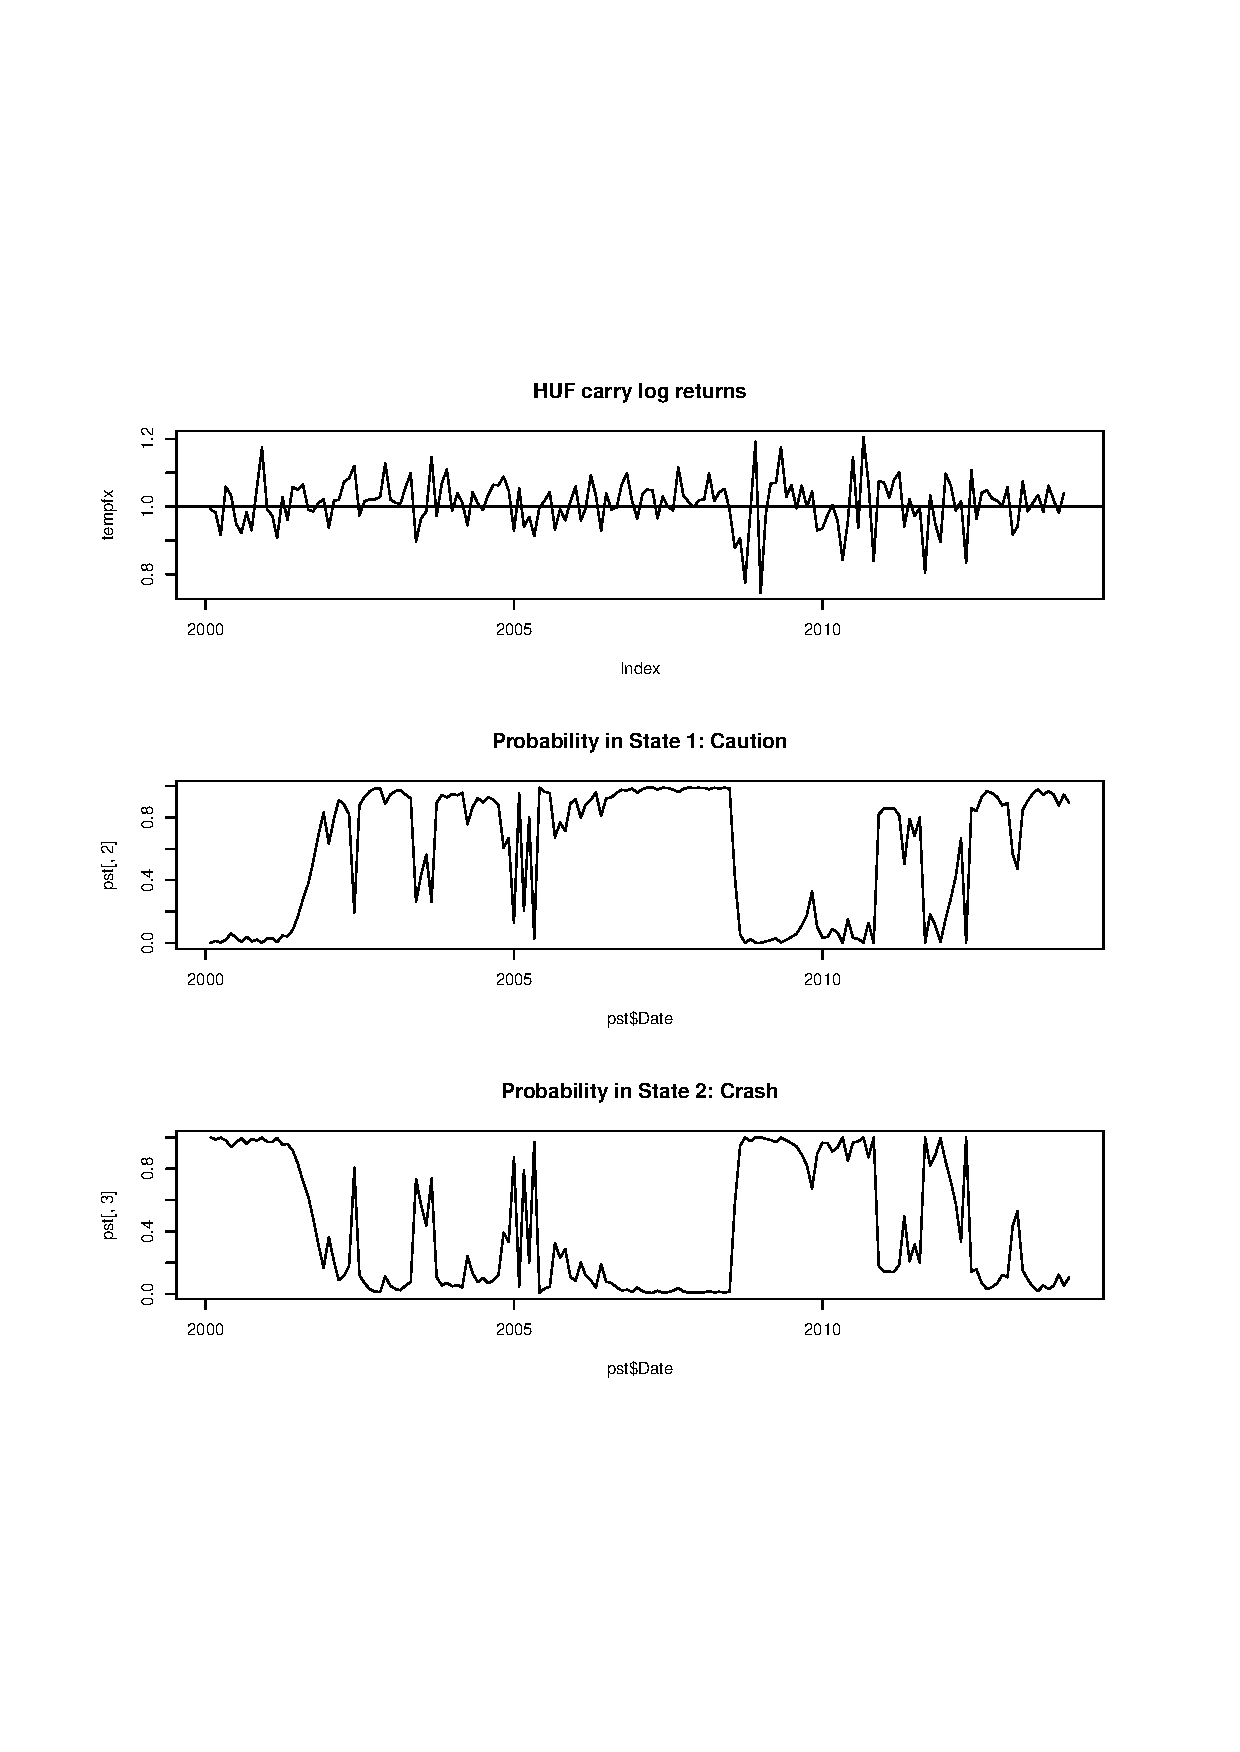
\includegraphics[scale = .50]{../../Figures/HUFEUR.pdf}
\caption{HUF Carry-trade probabilities}
\end{figure}

It is possible to read across the rows to assess the way that this probability changes as the VIX moves one and more standard deviations above and below is average.  For example, the first row reveals that there is a probability of about 8\% of a Hungarian crash when the VIX index is close to its mean. This rises to nearly 24\% when the VIX is one standard deviation above the mean and to over 52\% when the VIX is two standard deviations above its mean.  The probability of a crash is in the region of 80\% when the VIX is three standard deviations above the mean.  

\section{Conclusions}\label{secred:con}
In most cases investigated here, the carry-trade can be analysed as a system that switches between two states.  Most usually there are two states that can be characterised as being period of stable, when there are positive returns to the carry-trade and relatively low levels of conventional risk, or crash when there are losses and large risks.  This is consistent with the idea that international capital flows to emerging and transition economies are modelled most effectively periods of stable and then sudden stops.  There is little empirical support for a more nuanced three-regime model that would distinguish, within the period of stable, between periods of stable and periods of capital surge or speculative build up in addition to the crash. 

International risk aversion appears to influence carry-trade profits in many cases.  However, this influence is much more likely to affect the probability of switching from one regime to another than it is of directly affecting the level of carry-trade profits. 

The influence of measures of international risk aversion on the probability of moving from a state of stable to one of a crash is particularly likely to be seen in economies of central and eastern Europe.  It is much less prevalent in the more developed and more periphery countries under investigation like Turkey, Norway and Iceland. 

To be completed
\begin{itemize}
\item Pinning down the best model for Norway, Russia, Iceland and Turkey. Norway is either a one regime or three regime model; Iceland may be three.  Not sure about Russia and Turkey. 
\item Making the same assessment using US interest rates and the Ted-spread and assessing the relative vulnerability to each of these external factors. 
\item Looking at the dates when the crash takes place.  Which dates are the most common (Lehman's, Russian default et), which ones are unique to each country.  Ratio of international to domestic. 
\item Looking at the applicability of the two-regime model and levels of the openness of the financial system and the exchange rate regime.  
\end{itemize}




%Maximise $P(O \lambda)$, where $\lambda = (\pi, A, B)$.  The probability of observing sequence O for a given set of parameters.  The easiest way of doing this is to calculate the probability for each of the possible state sequences.  Consider one such sequence, $Q = q_1 q_2 \dots q_T$, the probability of the observed sequence for the state sequence Q is $P(O|Q \lambda) = \prod_{t = 1}^T P(O_t|q_t, \lambda)$.  If the observations are independent, this probability $P(O|Q \lambda)$ is equal to the probability of observing the outcome given the state, $b_{q_1}(O_1)\dot b_{q_2} (O_2) \dots b_{q_T}(O_T)$.  At each step, the forward variable $\alpha_t(i) = P(O_1 O_2 \dots O_t, q_t = S_i|\lambda)$ is calculated as the product of the sum of all the probability of each state for the previous period and the probability of transition from each of those states to the current as well as the product of being in this state given the observable. $\alpha_t(i)$ is the joint probability that observation is seen and state is achieved. 

\bibliography{../../../myrefsbackup}



\end{document}
